\subsection{Limitations of Perceptrons}

Connectionist neurons, or perceptrons, are limited in the variety of functions they are able to fit. 
When dealing with classification problems, a perceptron can only find a linear separation between any two classes. Irrespective of the neuron's non-linear activation function, the perceptron is regarded as a \emph{linear classifier}. Whether something falls on one side of the decision boundary or the other, is entirely based on applying a linear filter (i.e. $\vec w^{\top} \vec x$). The non-linearity $f(h)$ merely controls the value range of the neuron's response ($\{0,1\}, (-1,+1)$, \ldots) which helps in intepreting the neuron's response.\\

If observations for two different classes are dsitributed such that one cannot draw a line to separate them, then the two classes
are not linearly separable. In this case the perceptron will fail to find a suitable classification boundary between the two classes.


\begin{frame}\frametitle{Linear classifiers/linear decision boundaries}

Consider the following binary classification problems with $\vec x \in \R^2$.{}

\question{Can you find a line that separates the two classes for each case?}

\begin{figure}[h]
    \centering
	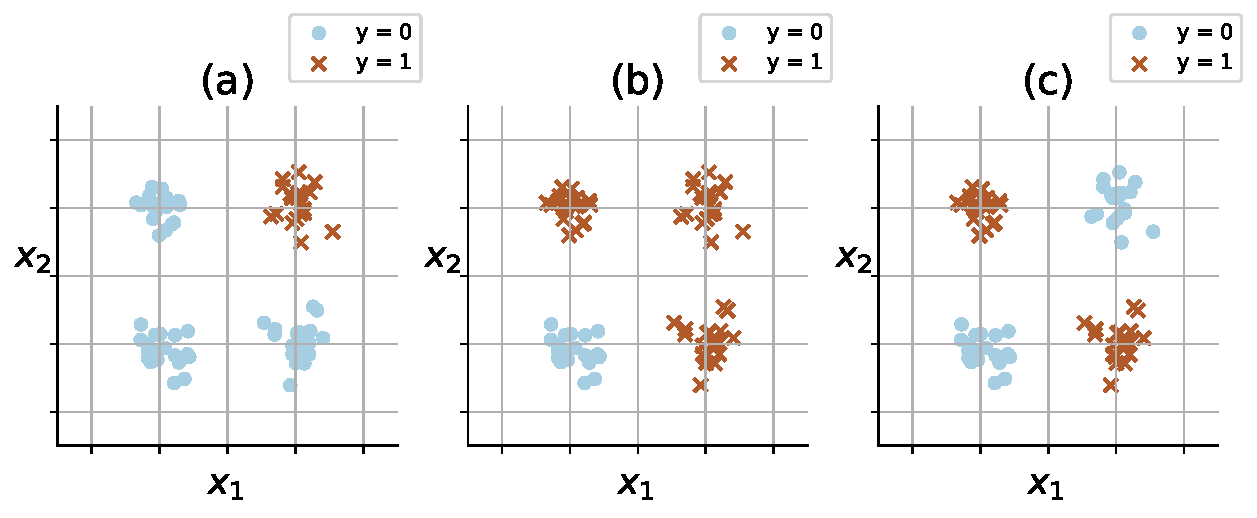
\includegraphics[width=0.8\textwidth]{img/and_or_xor_y}
	\caption{(a) points are classified according to the AND function,
	(b) points are classified according to the OR function,
	(c) points are classified according to the XOR function.
	}
	\label{fig:and_or_xor} 
\end{figure}


\end{frame}

\mode<article>{
In \figureref{fig:and_or_xor}, particularly (a) and (b),
it is possible to draw a line that separates the classes. Therefore, the AND and OR functions are linearly separable.
A perceptron is capable of finding such a separating line. However, this does not apply to the third case, for the XOR function.
It is impossible to find a single line that will separate the classes. The data from the XOR function is not linearly separable.
}

\begin{frame}
\question{Can we solve the XOR problem with multiple perceptrons? How?}

\slidesonly{
\begin{figure}[ht]
     \centering
	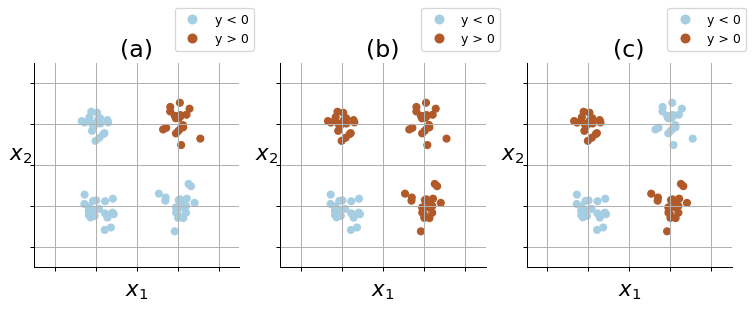
\includegraphics[trim=480 0 0 30, clip, width=0.4\textwidth]{img/and_or_xor_y.png}
	\caption*{A single perceptron can not solve the XOR problem.}
	\label{fig:xor} 
\end{figure}
}

\pause

\notesonly{
- Yes, Think of it as a divide and conquer approach. We split the XOR problem into mulitple sub-problems. 
A perecptron is used to solve each sub-problem.

If you're familiar with boolean algebra, you might reocgnize the following expression for the XOR function:
}

\begin{equation}
\label{eq:xor}
\mathrm{XOR}(x_1, x_2) = 
({\color{magenta}\,{x_1} \; \mathrm{AND} \; \overline{x}_2 \,})
 \;\; \mathrm{OR} \;\; 
({\color{green}\, \overline{x}_1 \; \mathrm{AND} \; x_2 \,})
\end{equation}

\end{frame}

%For instance, the first perceptron $S^1_1$ is tasked to separate the bottom-right cloud of points from the rest. 
%A second perceptron $S^1_2$ is used to separate the top-left cloud from the rest.
%A third perceptron $S^2_1$ will then use the responses from of the first two perceptrons, by responding to ``is only one of the two perceptrons ON?''.

%\figref{fig:build_xor} illustrates this approach. One need only recognize that each sub-problem is linearly separable.\\

%\begin{frame}
%\begin{figure}[ht]
    %\centering
	%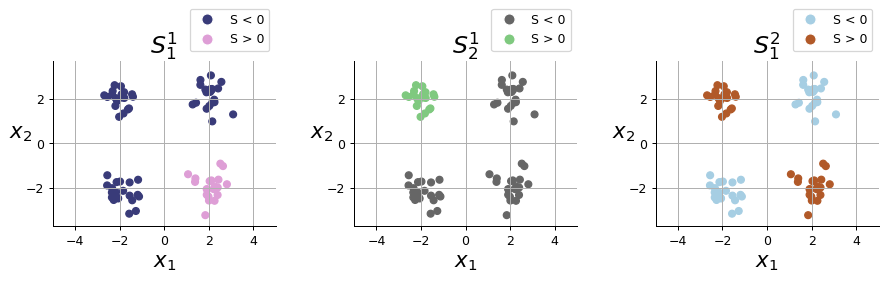
\includegraphics[width=0.9\textwidth]{img/build_xor.png}
	%\caption{Solving sub-problems of the XOR problem.}
	%\label{fig:build_xor} 
%\end{figure}

%What we are essentially describing is a Multilayered perceptron (MLP) with an architecture as illustrated in \figref{fig:xor_mlp_arch}. The MLP is made up of an output layer with  a single output neuron $S^2_1$, and one hidden layer with two hidden neurons, $S^1_1$ and $S^2_2$ (the superscript denotes the layer index, the subscript denotes the neuron index within its layer). The terms ``neurons'' and ``nodes'' will be used interchangeably and are treated as synonyms.

%\begin{figure}[ht]
    %\centering
	%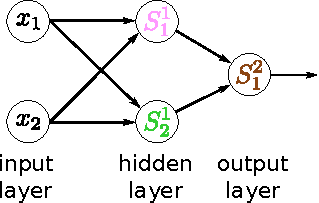
\includegraphics[width=0.5\textwidth]{img/xor_mlp_arch}
	%\caption{MLP architecture for the XOR problem consisting of one hidden layer with two hidden nodes $S^1_1$, $S^1_2$, and one output layer with a single output neuron $S^2_1$}
	%\label{fig:xor_mlp_arch} 
%\end{figure}

%\end{frame}

%\section{Classes of neural networks}
%\begin{frame}

%hello

%\end{frame}
